\documentclass{article}
\usepackage{lastpage}
\usepackage[polish]{babel}
\usepackage[T1]{fontenc}
\usepackage[utf8]{inputenc}
\usepackage{graphicx}
\usepackage{fancyhdr}
\usepackage{xstring}
\usepackage{xcolor}
\usepackage{indentfirst}
\usepackage[none]{hyphenat}
\usepackage{subfig}
\usepackage{float}

\newcommand{\version}{v1.0.4}
\newcommand{\lastPage}{19}
\newcommand{\tab}{\hspace{1cm}}
\newcommand{\justy}[1]{
\StrSubstitute{#1}{ }{ \hfill}

}


\pagestyle{fancy}
\setlength
\headheight{40pt}
\renewcommand{\footrulewidth}{0.4pt}
\fancyhf{}

\rhead{Dokumentacja projektu}
\lhead{
\includegraphics[width=5cm]{images/pp.jpg}\newline Wydział informatyki i telekomunikacji}

\lfoot{Politechnika Poznańska}
\cfoot{Page \thepage\space of\space \lastPage}
\rfoot{19.03.2020r.}

\begin{document}
\begin{titlepage}
		\begin{center}
			
						\LARGE
			Politechnika Poznańska
			
			\vspace{0.3cm}
			
			\large
			Wydział informatyki i telekomunikacji
			
			\vspace{3.0cm}
			\huge
			\textbf{Dokumentacja projektu}
			
			\vspace{0.5cm}
			
			\large
			Dokumentacja projektu z zajęć Telefonia IP
			
			\vspace{2.4cm}
			
			\LARGE
			\textbf{Autorzy:}
			
			\vspace{0.3cm}
			
			Adrian Golczak 136239
			adrian.e.golczak@student.put.poznan.pl
			
			\vspace{0.3cm}
			
			Marcin Kubiak 136267
			marcin.w.kubiak@student.put.poznan.pl
			
			\vfill
			
			\normalsize
			Wersja: \version
			
			\vspace{2cm}
			

			
			19.03.2020 r.
			
		\end{center}
\end{titlepage}
\tableofcontents
\newpage
	\section{Charakterystyka ogólna projektu}
	\tab Przedmiotem projektu pn. 'Opracowanie bezpiecznego systemu komunikacji głosowej w sieci IP (VoIP) wraz z jego implementacją' jest opracowanie aplikacji mobilnej wyposażonej w odpowiednie algorytmy umożliwiające bezpieczną rozmowę pomiędzy dwoma użytkownikami aplikacji. Główną koncepcją projektu jest stworzenie tzw. poczekalni, w której zalogowani użytkownicy bedą mogli się łączyć z kim tylko chcą i odbywać z nim rozmowę. Aplikacja będzie spełniała zasady integralności i poufności, aby uniemożliwić podsłuchanie rozmowy przez osobę trzecią.

	\section{Architektura systemu}
	\subsection{Uproszczona architektura technologii}
\tab Funkcjonalnie, możliwe będzie połączenie dwóch clientów aplikacji mobilnej poprzez server napisany w spring boot framework.\\
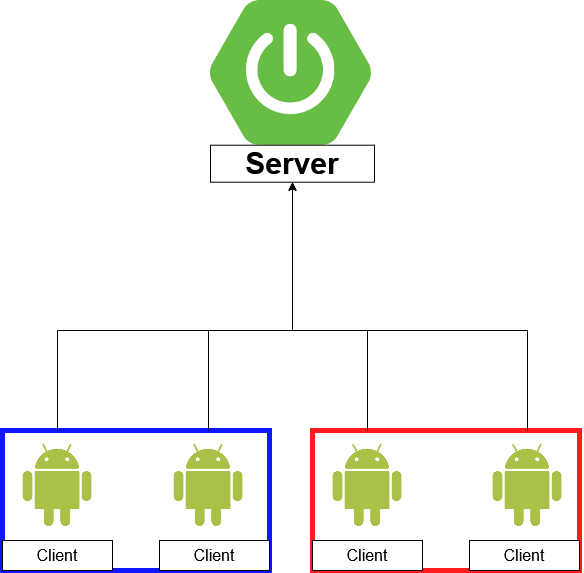
\includegraphics[width=12cm]{images/simple architecture.png}
\begin{center}
	\footnotesize
	Rysunek 1. Uproszczona architektura systemu
\end{center}
\subsection{Architektura przepływu}
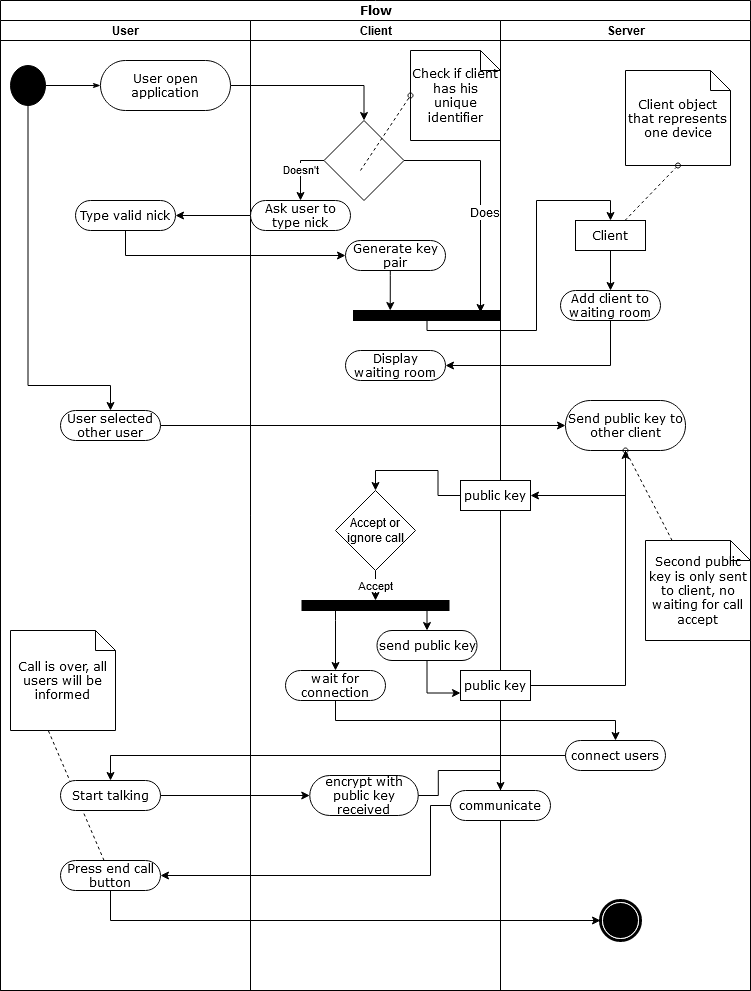
\includegraphics[width=12cm]{images/flow.png}
\begin{center}
	\footnotesize
	Rysunek 2. Architektura przepływu komunikacji pomiedzy użytkownikiem, klientem, a serwerem.
\end{center}
	\section{Wymagania}
	\justy{Poniżej opisane zostaną wymagania funkcjonalne i niefunkcjonalne aplikacji, z wyróżnieniem różnych stanów użytkownika.}
	\subsection{Funkcjonalne}
	\tab funkcjonalne
	\subsection{Niefunkcjonalne}
	\begin{itemize}
\item łączenie dwóch użytkowników,
\item generowanie ID sesji
\item negocjacje klucza o rozmiarze 256 bitów na potrzeby AES-256,
\item szyfrowanie rozmowy wykorzystując AES-256,
\item minimalna wersja systemu Android: 10.0.0,
\item brak wymogu podania hasła przez użytkownika przy logowaniu,
\item limit użytkowników w poczekalni podyktowany mocą obliczeniową serwera,
\item jedno urządzenie mobilne to jedna instancja klienta,	\item w ramach jednego pokoju może przebywać jedynie dwóch użytkowników,
\item zmiana głośności rozmowy za pomocą wbudowanych funckji sprzętowych urządzenia.
\end{itemize}

	\section{Technologie, narzędzia, środowisko, biblioteki, kodeki}
	\begin{itemize}
	\item \textit{TeXstudio}
	\item \textit{InteliJ}
	\item \textit{Java11}
	\item \textit{SpringBoot}
	\item \textit{AndroidStudio}
	\item \textit{javax.sound}
\end{itemize}
	\section{Opis najważniejszych protokołów}
	\justy{W tej sekcji opiszemy najważniejsze protokoły zawarte w naszym projekcie.}

\subsection{Dołączanie użytkownika do poczekalni}

\justy{Po uruchomieniu aplikacji użytkownik ma za zadanie wpisać swój pseudonim. Następnie wysyłane jest żądanie do serwera o dołączenie do poczekalni, które składa się z wylosowanego przez klienta klucza publicznego oraz jego pseudonimu. Serwer następnie dodaje użytkownika do poczekalni i nadaje mu unikalny identyfikator, na którym opiera się komunikacja z pozostałymi użytkownikami.}

\subsection{Łączenie użytkowników oraz negocjacje klucza}
\justy{W momencie gdy użytkownik pragnie się połączyć z inną osobą w poczekalni wysyła on żądanie do serwera. Ten tworzy sesję i dołącza do niej użytkownika próbującego się połączyć (inicjującego połączenie). Jeśli osoba odbierająca przyjmie połącznie to serwer dołącza ją do sesji i wysyła odpowiednie komunikaty zawierające klucze publiczne potrzebne do wylosowania 256 bitowego klucza AES po 128 bitów każdy. Obie strony rozmowy wymieniają się zaszyfrowanymi częściami klucza. Po potwierdzeniu otrzymania części klucza przez drugą stronę rozpoczyna się szyfrowana komunikacja między dwoma użytkownikami.}
	\section{Ekrany}
	\justy{Poniżej zaprezentowano wstępne makiety ekranów jakie będą używane w aplikacji mobilnej, do obsługi dodawania użytkownika do kolejki, dzwonienia, odbierania połączeń, rozmowy i kończenia rozmowy. Wszystkie ekrany są jedynie koncepcją interfejsu i nie należy traktować ich jako produktu końcowego.}
\hfil


\begin{figure}[H]
	\centering
	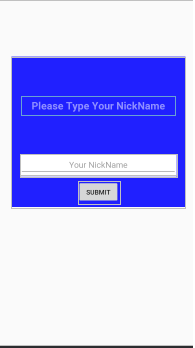
\includegraphics[width=8cm]{images/5.png}
	\caption{\centering Pierwszy ekran z prośbą o podanie pseudonimu użytkownika.}
	\hfill 
\end{figure} 
\begin{figure}[H]
	\centering
	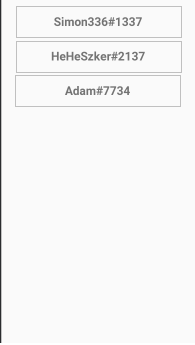
\includegraphics[width=8cm]{images/1.png}
	\caption{\centering Ekran z widoczną ''poczekalnią'', w której znajduje się trzech użytkowników.}
	\hfill 
\end{figure} 
\begin{figure}[H]
	\centering
	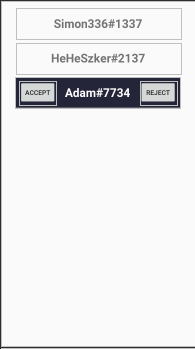
\includegraphics[width=8cm]{images/2.png}
	\caption{\centering Informacja o nadchodzącym połączenia od użytkownika Adam.}
	\hfill 
\end{figure} 
\begin{figure}[H]
	\centering
	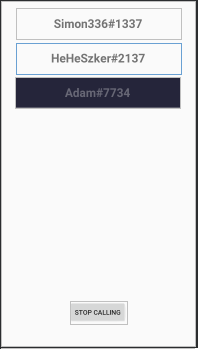
\includegraphics[width=8cm]{images/3.png}
	\caption{\centering Próba połączenia się z użytkownikiem Adam.}
	\hfill 
\end{figure} 
\begin{figure}[H]
	\centering
	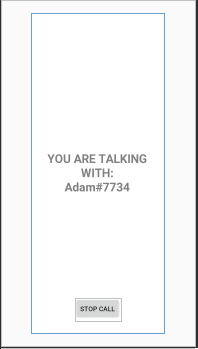
\includegraphics[width=8cm]{images/4.png}
	\caption{\centering Rozmowa z użytkownikiem Adam.}
	\hfill 
\end{figure}
\hfill

	\section{Diagramy UML}
	{W tym rozdziale skupimy się na 4 typach diagramów UML: przypadków użycia, przebiegów, stanów oraz klas.}
	\subsection{Diagram przypadków użycia}
	\vspace{0.5cm}
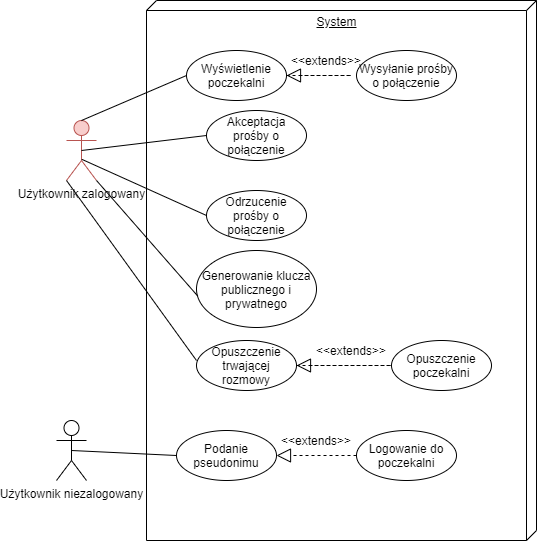
\includegraphics[width=\textwidth]{images/TIP-diagramPU.png}	
\caption{Rysunek 1: Diagram przypadków użycia z podziałem na dwóch aktórów: użytkownika zalogowanego i niezalogowanego}





	\subsection{Uproszczony diagram przepływu}
	\justy{Poniżej zaprezentowano uproszczony diagram przepływu. Diagram podzielono na 3 obiekty: użytkownika aplikacji, klienta, czyli aplikację mobilną będącą pośrednikiem pomiędzy użytkownikiem, a serwerem, i serwer który obsługuje wszystkie zapytania i odpowiednio je przetwarza, zarządza sesjami i połączeniami.}

\begin{figure}[H]
	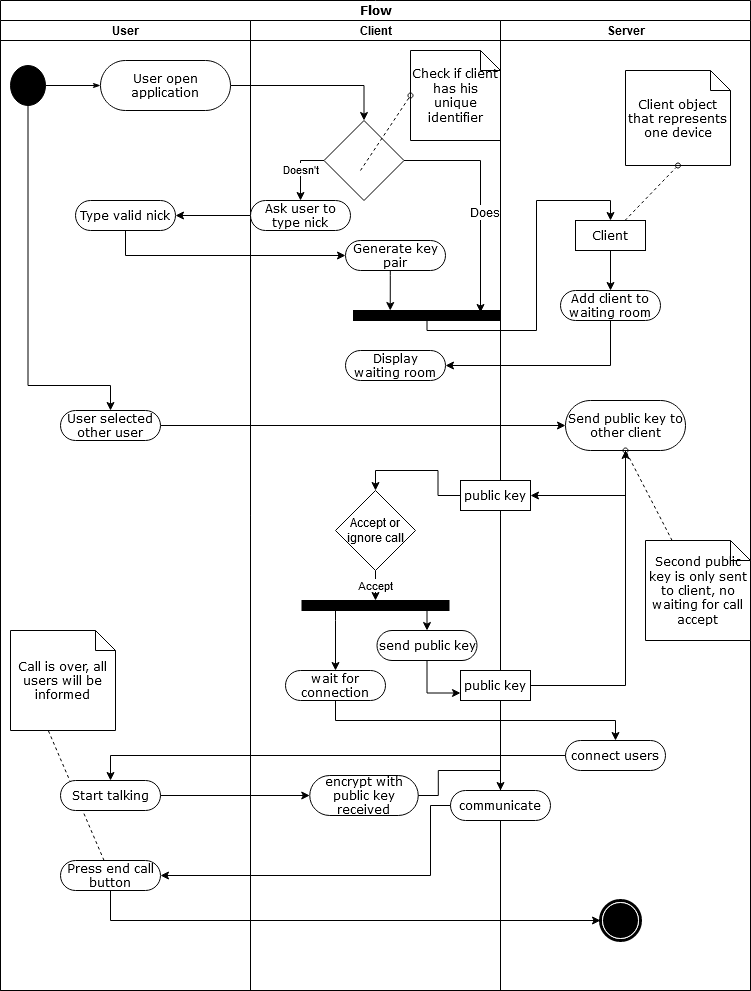
\includegraphics[width=\textwidth]{images/flow.png}
	\centering	
	\caption{\centering Uproszczony diagram przepływu przedstawiajacy inicjalizację sesji, a także dodania użytkownika do poczekalni.}
\end{figure}
	\subsection{Diagramy stanów}
	\begin{figure}[H]
	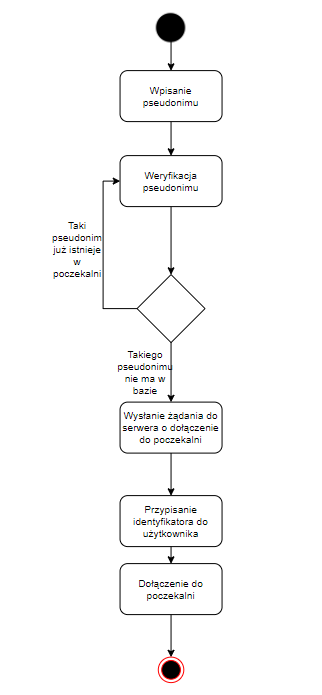
\includegraphics[width=0.5\textwidth]{images/stan1.png}
	\centering	
	\caption{\centering Diagram stanu dla dołączania użytkownika do poczekalni.}
\end{figure}

\begin{figure}[H]
	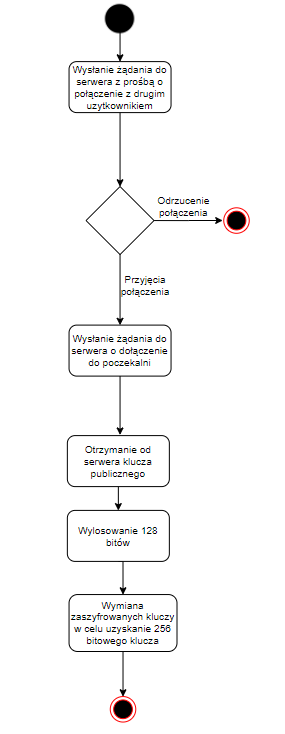
\includegraphics[width=0.5\textwidth]{images/stan2.png}
	\centering	
	\caption{\centering Diagram stanu dla łączenia użytkowników i negocjacji klucza między nimi.}
\end{figure}
	\subsection{Diagram klas}
	\justy{Poniżej prezentujemy 6 diagramów klas klienta i 6 diagramów klas serwera.}

\subsubsection{Diagramy klas klienta}
\begin{figure}[H]
	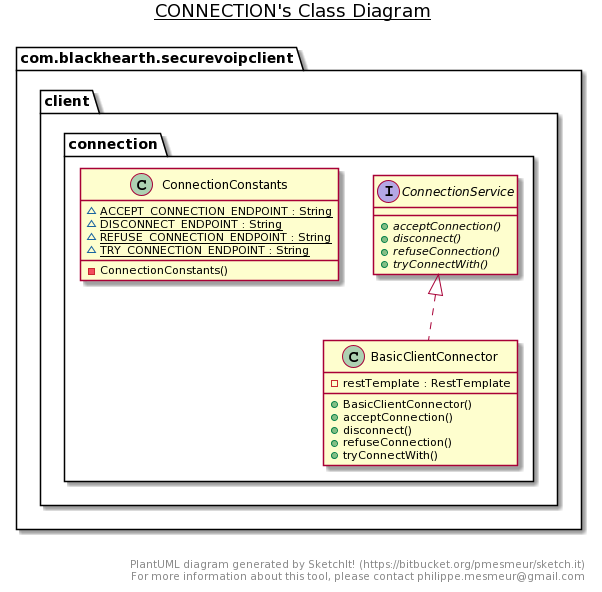
\includegraphics[width=0.5\textwidth]{images/uml/1.png}
	\centering	
	\caption{\centering Diagram klas serwisu łączącego dwóch klientów.}
\end{figure}
\begin{figure}[H]
	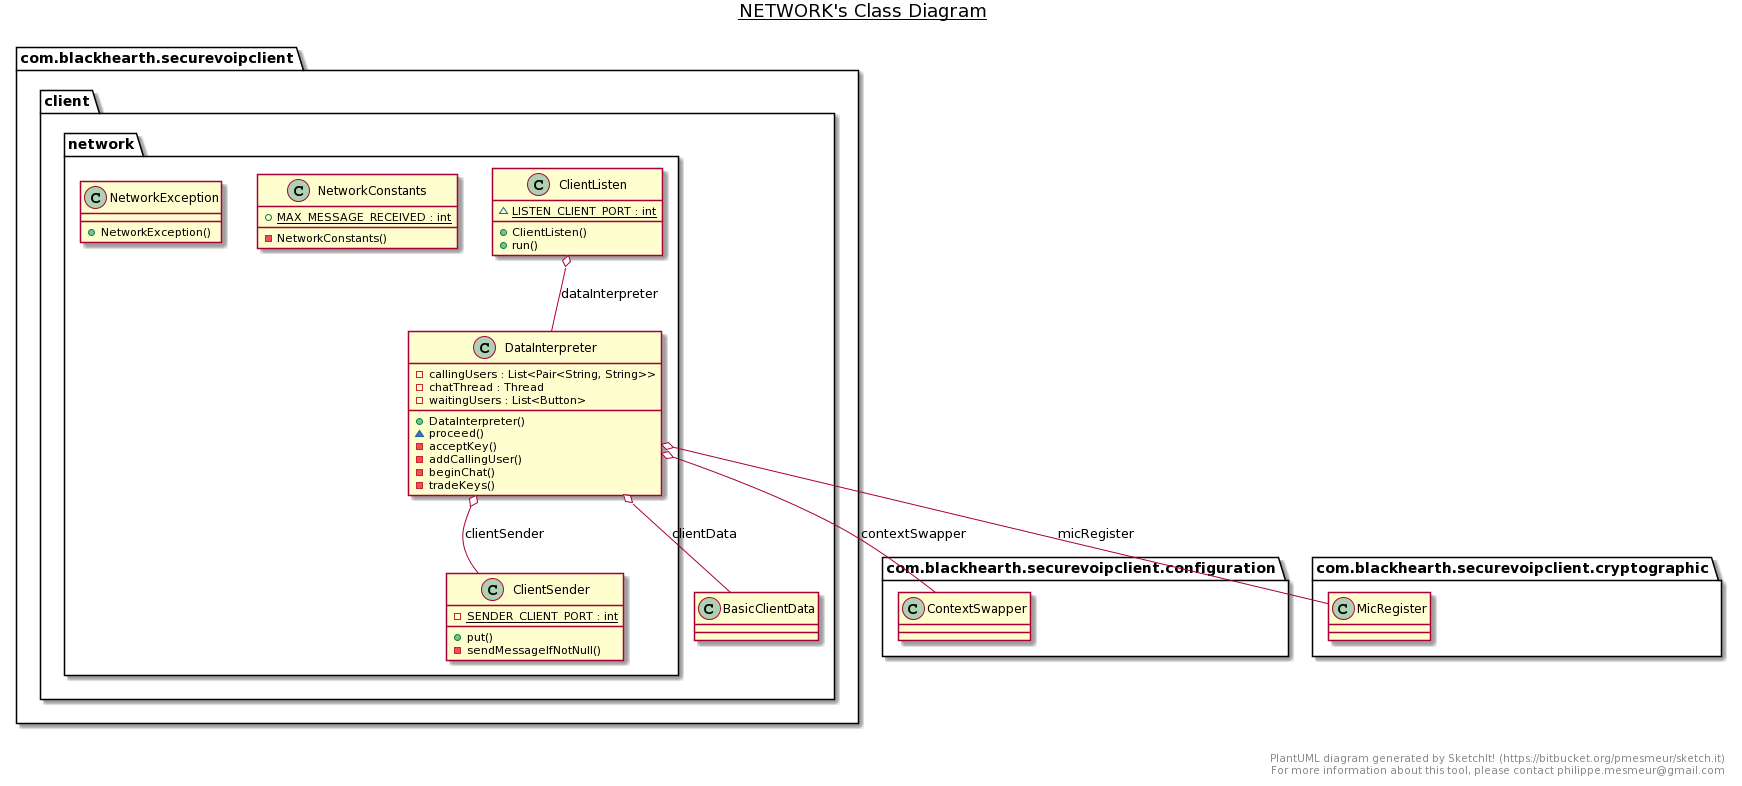
\includegraphics[width=0.5\textwidth]{images/uml/2.png}
	\centering	
	\caption{\centering Diagram klas połączenia UDP pomiędzy dwoma klientami.}
\end{figure}
\begin{figure}[H]
	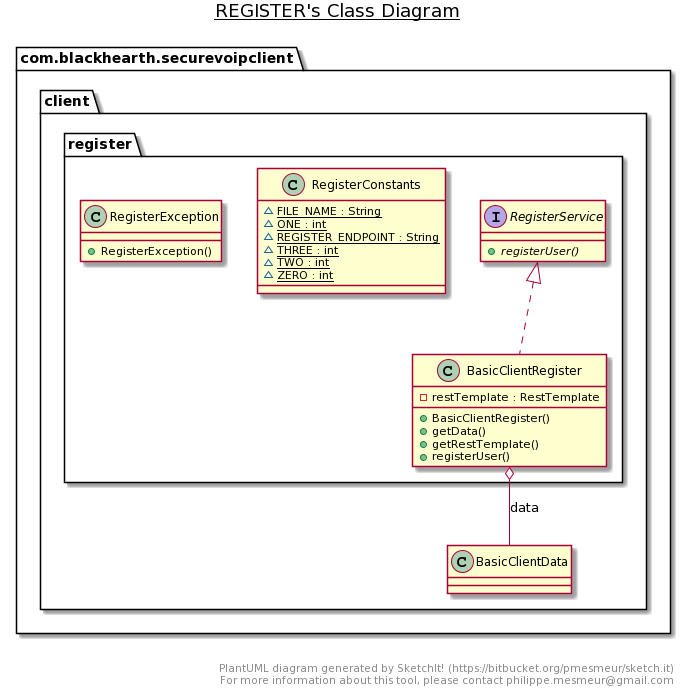
\includegraphics[width=0.5\textwidth]{images/uml/3.png}
	\centering	
	\caption{\centering Diagram klas sewrisu rejestrującego nowego użytkownika.}
\end{figure}
\begin{figure}[H]
	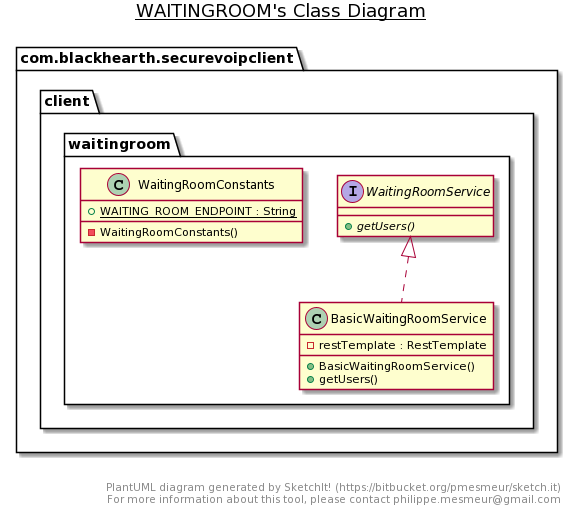
\includegraphics[width=0.5\textwidth]{images/uml/4.png}
	\centering	
	\caption{\centering Diagram klas serwisu pobierającego listę użytkowników z serwera.}
\end{figure}
\begin{figure}[H]
	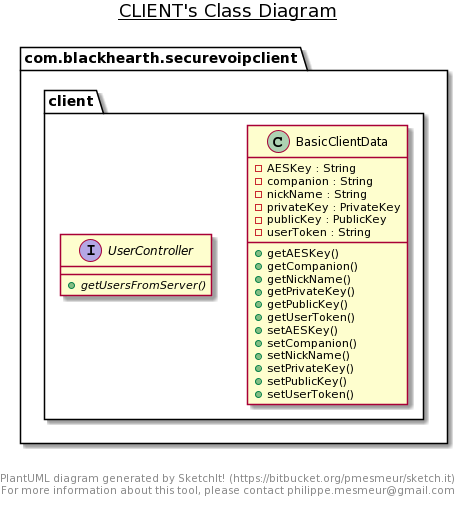
\includegraphics[width=0.5\textwidth]{images/uml/5.png}
	\centering	
	\caption{\centering Diagram klas danych użytkownika.}
\end{figure}
\begin{figure}[H]
	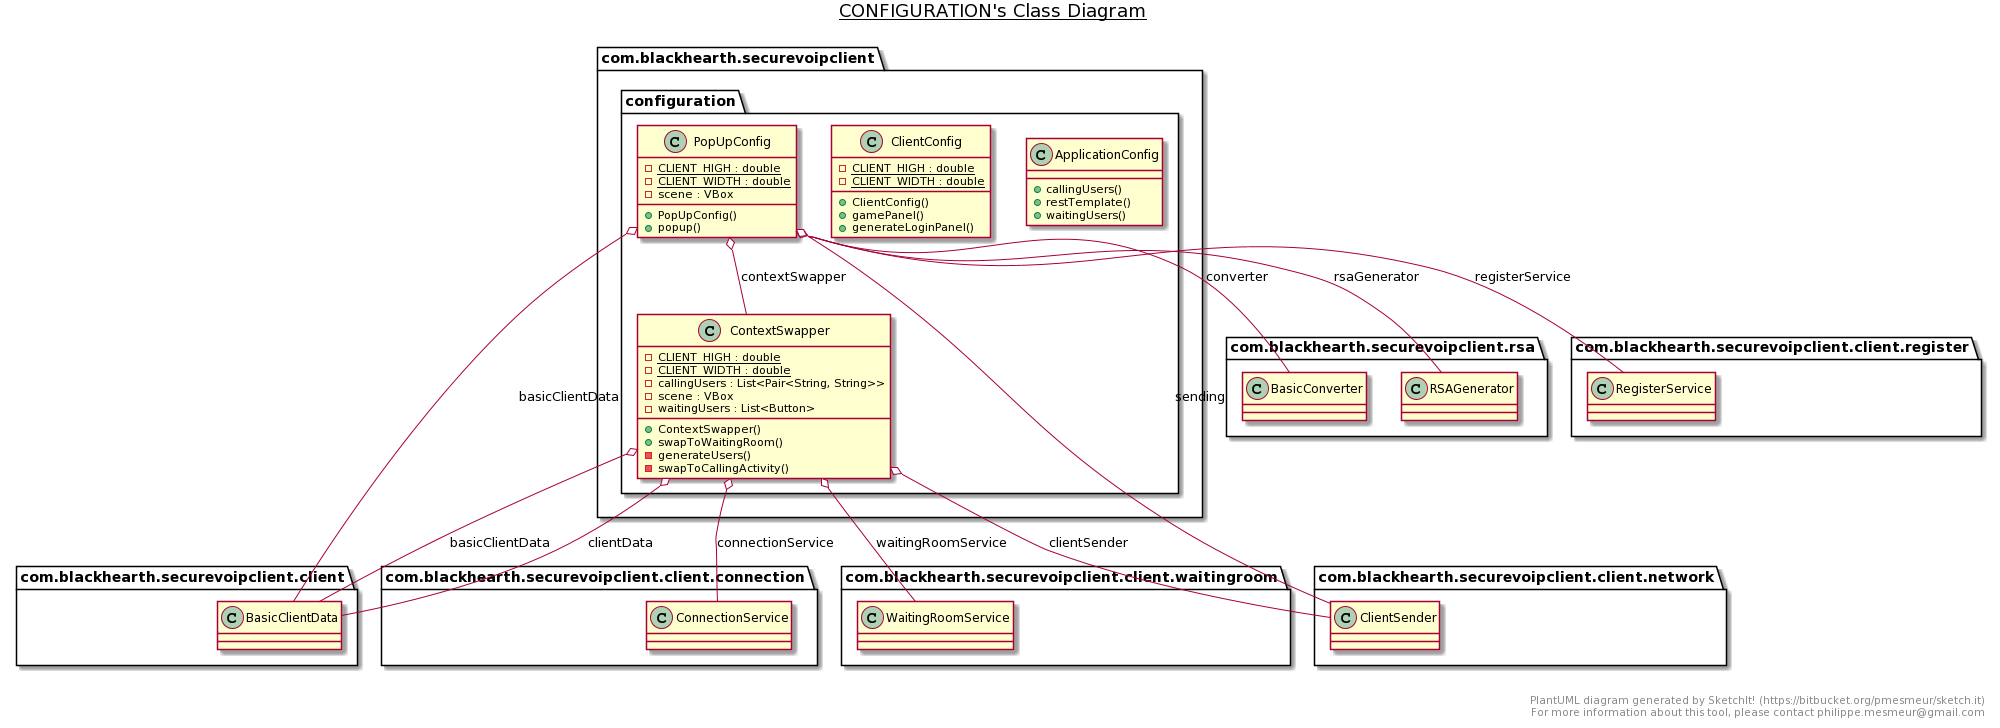
\includegraphics[width=0.5\textwidth]{images/uml/6.png}
	\centering	
	\caption{\centering Diagram klas konfiguracji klienta.}
\end{figure}

\subsubsection{Diagramy klas serwera}
\begin{figure}[H]
	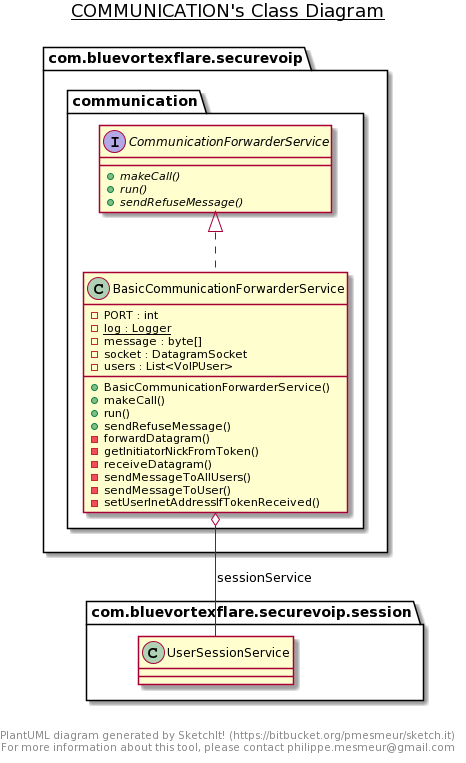
\includegraphics[width=0.5\textwidth]{images/uml/s1.png}
	\centering	
	\caption{\centering Diagram klas połączenia UDP pomiędzy serwerem a klientem.}
\end{figure}
\begin{figure}[H]
	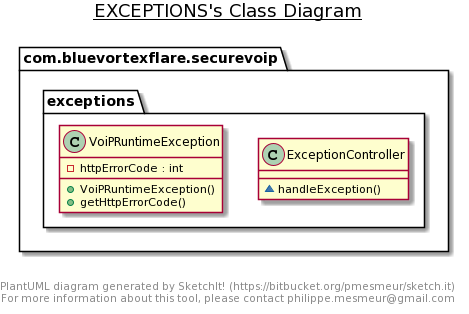
\includegraphics[width=0.5\textwidth]{images/uml/s2.png}
	\centering	
	\caption{\centering Diagram klas wyjątków serwera.}
\end{figure}
\begin{figure}[H]
	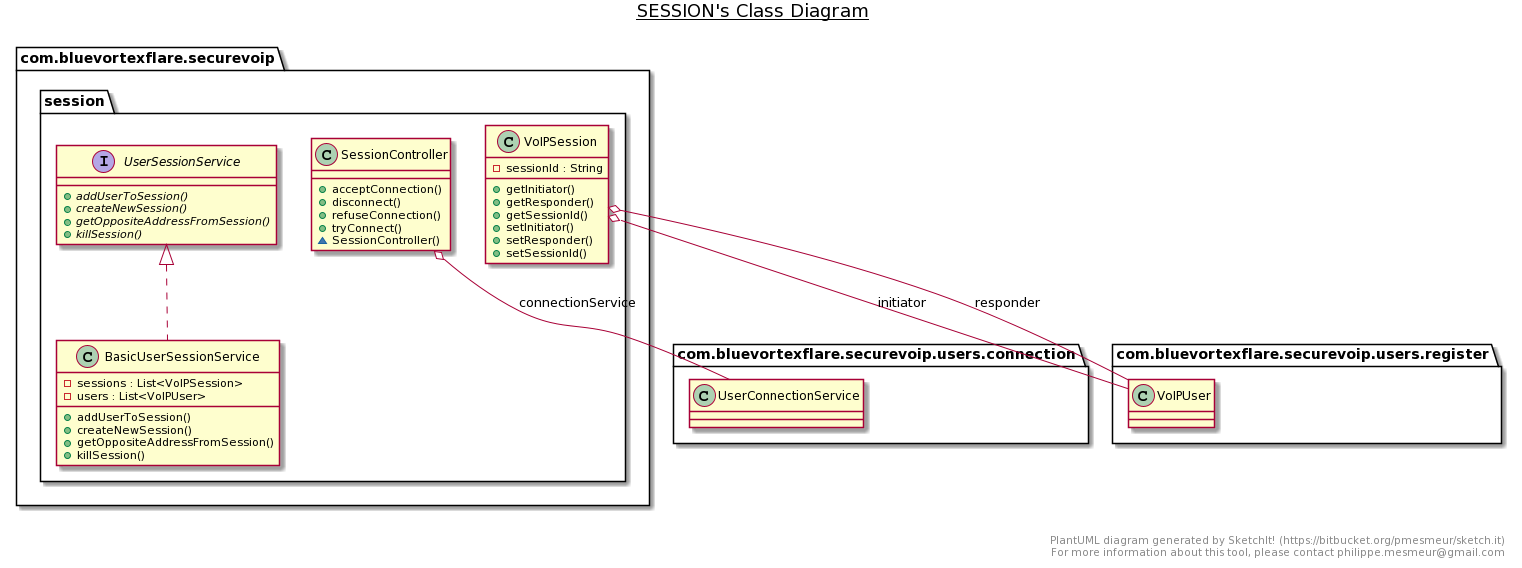
\includegraphics[width=0.5\textwidth]{images/uml/s3.png}
	\centering	
	\caption{\centering Diagram klas serwisu zarządzającego sesjami użytkowników.}
\end{figure}
\begin{figure}[H]
	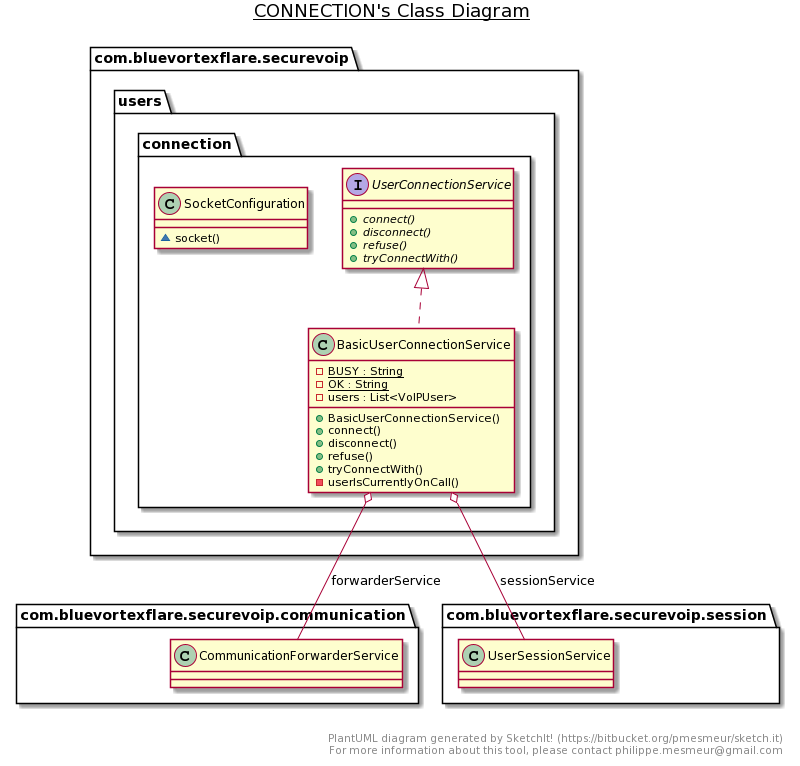
\includegraphics[width=0.5\textwidth]{images/uml/s4.png}
	\centering	
	\caption{\centering Diagram klas serwisu zarządzającego połączeniem pomiędzy użykownikami.}
\end{figure}
\begin{figure}[H]
	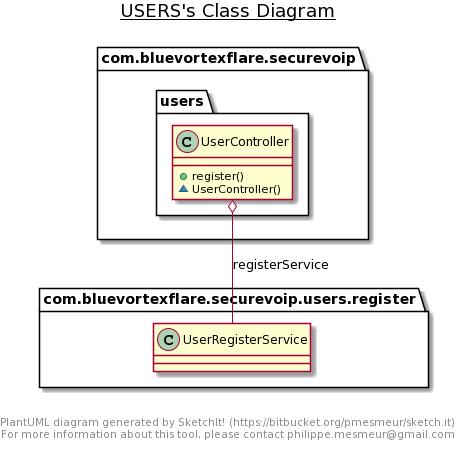
\includegraphics[width=0.5\textwidth]{images/uml/s5.png}
	\centering	
	\caption{\centering Diagram klas ilustrujący zależność pomiędzy kontrolerem użytkownika, a serwisem rejestrującym.}
\end{figure}
\begin{figure}[H]
	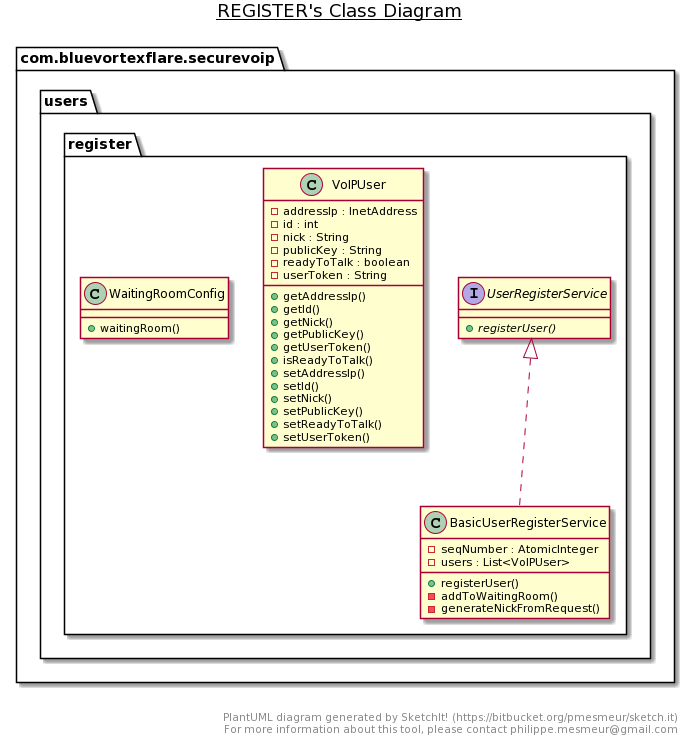
\includegraphics[width=0.5\textwidth]{images/uml/s6.png}
	\centering	
	\caption{\centering Diagram klas serwisu rejestrującego.}
\end{figure}
	\section{Implementacja serwera}
	\justy{W tej sekcji prezentujemy najciekawsze fragmenty kodu aplikacji serwerowej. Jako wzorzec projektowy do wytwarzania oprogramowania użyliśmy Domain Driven Design, dzięki czemu podzieliliśmy kod na domeny, a to pozwoliło utrzymać go w ''czystości'' i ułatwia ewentualną późniejszą rozbudowę.}

\subsection{RegisterService}
\just{Serwis ten ma za zadanie zarządzać poczekalnią, dodawać i usuwać z niej użytkowników. Poczekalnia jest wstrzykniętą listą użytkowników przy użyciu Inversion of Controll Container'a, jako implementacji Dependency Injection.}

\begin{figure}[H]
	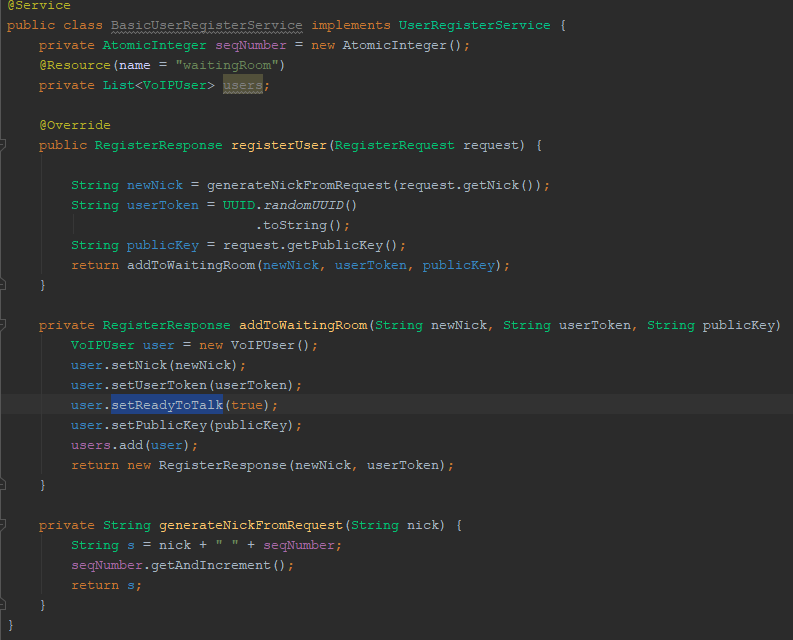
\includegraphics[width=\textwidth]{images/code1.png}
	\centering	
	\caption{\centering Kody serwisu zarządzającego użytkownikami i poczekalnią.}
\end{figure}

\subsection{ConnectionService}
\justy{Serwis odpowiedzialny za łączenie i rozłączanie użytkowników pośrednio wykorzystuje SessionService który zarządza dodatkowo sesjami użytkowników.}

\begin{figure}[H]
	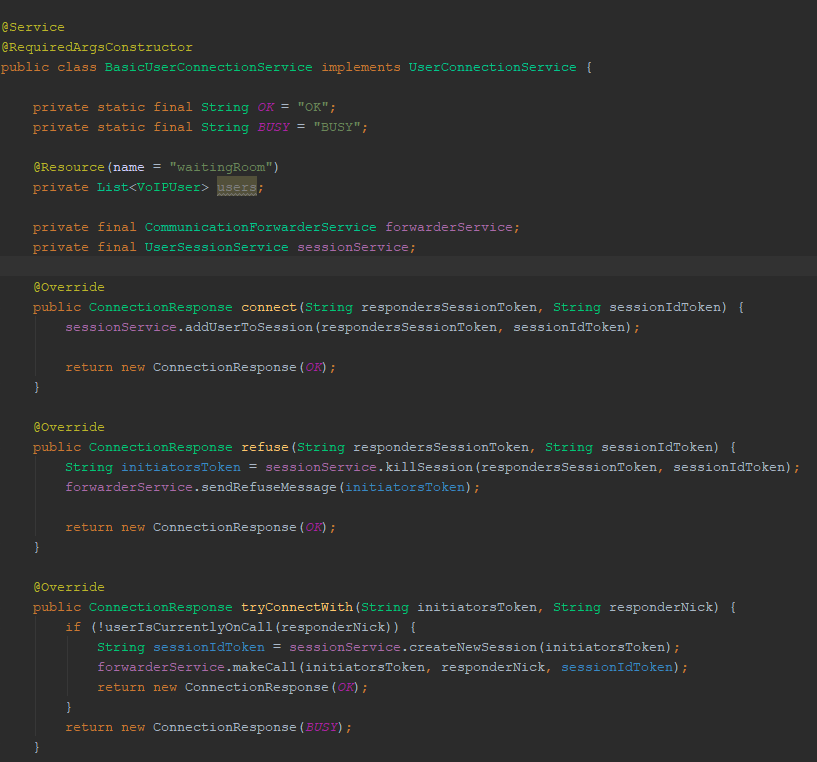
\includegraphics[width=\textwidth]{images/code2.png}
	\centering	
	\caption{\centering Klasa zarządzająca połączeniem użytkowników podczas próby rozmowy.}
\end{figure}
	\section{Implementacja klienta}
	
W tej sekcji ukazujemy fragmenty kodu aplikacji klienta napisanych w języku Java.

\subsection{AudioConstants}
Klasa przechowująca stałe wykorzystywane do odbioru jak i przesyłania dzwięku w postaci bajtów.

\begin{figure}[H]
	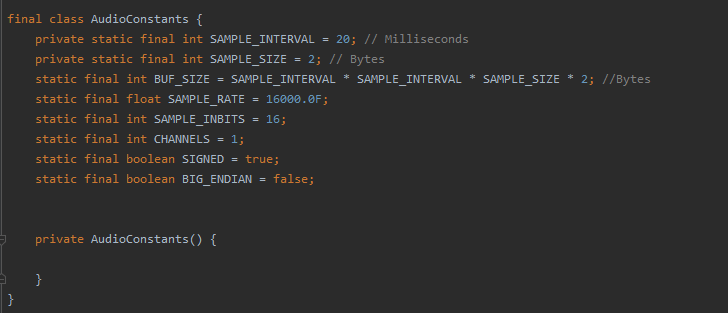
\includegraphics[width=\textwidth]{images/code3_1.png}
	\centering	
	\caption{\centering Stałe wykorzystywane przy cyfrowej obróbce dzwięku.}
\end{figure}


\subsection{BasicMicRegister}
Konstruktor tworzący obiekty potrzebne do otrzymywania jak i wysyłania dzwięku z mikrofonu jak i do szyfrowania i deszyfrowania ciągu bitów.

\begin{figure}[H]
	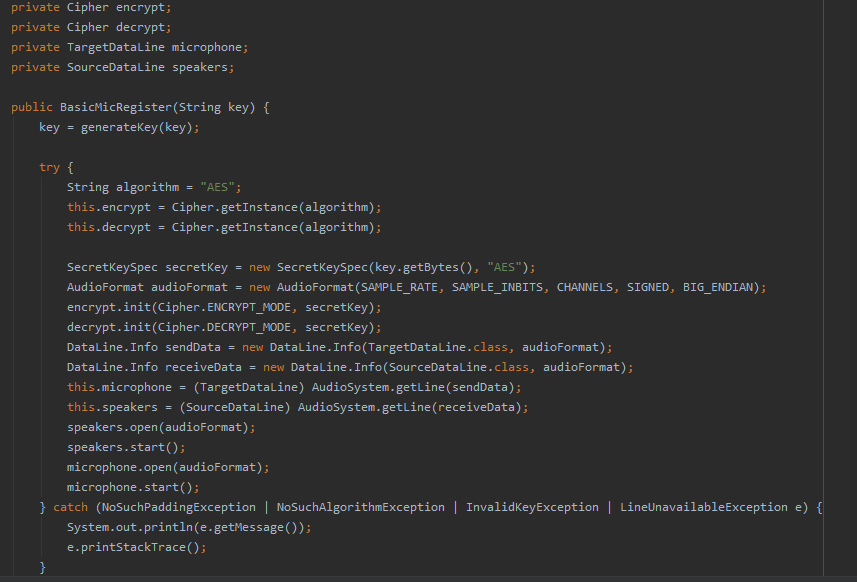
\includegraphics[width=\textwidth]{images/code4.png}
	\centering	
	\caption{\centering Konstruktor BasicMicRegister.}
\end{figure}


\subsection{sendVoiceMessage}
Metoda odpowiedzialna za przesyłanie zaszyfrowanej wiadomości głosowej uprzednio ustalonym kluczem szyfru blokowego AES 256.

\begin{figure}[H]
	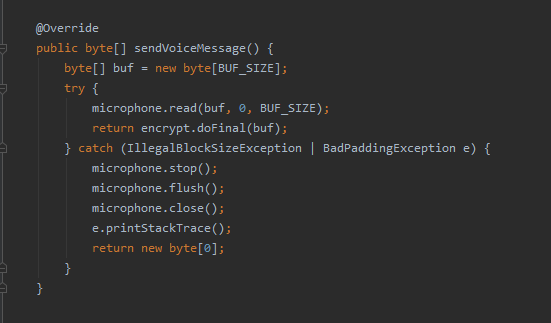
\includegraphics[width=\textwidth]{images/code5.png}
	\centering	
	\caption{\centering Metoda odpowiedzialna za przesyłanie zaszyfrowanej wiadomości.}
\end{figure}

\subsection{receiveMessage}
Metoda odpowiedzialna za odbieranie zaszyfrowanej wiadomości głosowej oraz odszyfrowanie jej i przekazaniu jej głośnikowi w celu odtworzenia dzwięku.
\begin{figure}[H]
	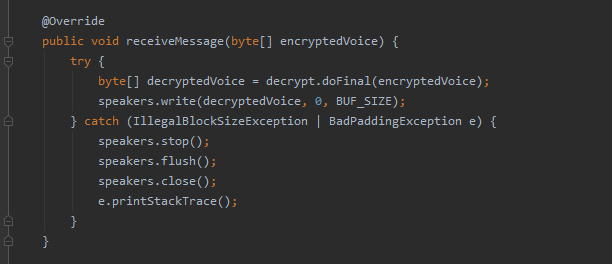
\includegraphics[width=\textwidth]{images/code6.png}
	\centering	
	\caption{\centering Metoda receiveMessage.}
\end{figure}
	\section{Testy i przebieg sesji}
	coś
	\section{Analiza bezpieczeństwa}
	coś
	\section{Podsumowanie}
	\justy{Na przestrzeni pisania projektu napotkaliśmy na wiele problemów natury technologicznej jak i mocy obliczeniowej. Z początku planowana aplikacja mobilna stała się aplikacją desktopową, gdyż Android Studio sprawił nam za dużo problemów, a Java i JavaFX to pojęcia nam znane. Osiągnęliśmy to, co chcieliśmy. Udało nam się połączyć dwie aplikacje klienckie ze sobą, aby miały możliwość ze sobą się komunikować. Niestety, jakość połączenia nie jest satysfakcjonująca, która wynika najprawdopodobniej z wykorzystania nieodpowiednich klas, więc jest to jedna z funkcjonalności, którą chcielibyśmy poprawić w najbliższej przyszłości, żeby móc rozmawiać płynnie i bez strat pakietów. }
	\section{Podział prac}
	Projekt został wykonany z często wspólnymi obowiązkami, podział prac prezentuje się następująco:

\noindent Adrian Golczak: 
\begin{itemize}
	\item nadzorowanie prac projektu,
	\item pisanie dokumentacji projektu,
	\item stworzenie szkieletu serwera oraz klienta,
	\item napisanie metod umożliwiających łączenie się użytkowników z serwerem, poczekalnią oraz samym sobą,
	\item stworzenie ekranów poczekalni, rozmowy.
\end{itemize}
Marcin Kubiak:
\begin{itemize}
	\item pisanie dokumentacji projektu,
	\item generowanie klucza publicznego, prywatnego,
	\item przetwarzanie wysyłanych i odbieranych bajtów.	
\end{itemize}

\subsection{Cele zrealizowane}
\justy{Z pewnością udała nam się negocjacja klucza AES 256 między użytkownikami rozpoczynającymi rozmowę, dodatkowo szyfrowanie i deszyfrowanie bajtów również działa prawidłowo. W trakcie prac udało się uzyskać połączenie między użytkownikami znajdującymi się w tej samej sieci, a sama rozmowa przebiega prawidłowo.}
\subsection{Cele niezrealizowane}
\justy{Nie udało nam się stworzyć aplikacji mobilnej tak jak wcześniej zakładaliśmy, przez co zabrakło czasu na dopracowanie pewnych elementów działającej aplikacji klienckiej opartej na JavaFX.}
\subsection{Napotkane problemy}
\justy{Pisząc aplikację mobilną w pewnym momencie wszystkie funkcjonalności systemu zaczęły generować mnóstwo błędów, żeby to naprawić musielibyśmy od zera cały szkielet kodu aplikacji klienckej zmienić, lepszym sposobem było przejście na aplikację desktopową, gdyż Android Studio sprawiał mnóstwo problemów, a sam emulator zajmował dużo pamięci RAM przez co testowanie aplikacji było bardzo problematyczne i lepszą opcją było przejście na JavaFX.}
\subsection{Perspektywa rozwoju}
\justy{Myślę, że w niedalekiej przyszłości warto zaimplementować algorytm logowania oraz odzyskiwania hasła. Dodatkowo można rozszerzyć funkcjonalność aplikacji klienckiej o czat tekstowy w celu np. wysyłania linków.}
\end{document}
